\documentclass{aamas2012}
% Setting letter size with pdflatex
\pdfpagewidth=8.5truein
\pdfpageheight=11truein

\usepackage{makeidx}
\usepackage{amsmath}   
\usepackage{amsfonts}   
\usepackage[retainorgcmds]{IEEEtrantools}
\usepackage{thumbpdf}
\usepackage{multicol}   
\usepackage{graphicx}   
\usepackage{listings}
\usepackage{algorithm}
\usepackage{algorithmic}
\usepackage{tikz}
\usepackage{subfigure}

\usepackage{hyperref}
\hypersetup{ 
  pdftitle          = {Learning in a Small World},
  pdfauthor         = {Arun Tejasvi Chaganty, Prateek Gaur, Balaraman Ravindran},
  colorlinks        = true,
  linkcolor         = red,
  urlcolor          = red
  citecolor         = blue,
}

% Section References
\newcommand{\secref}[1] {\hyperref[#1]{Section~\ref*{#1}}}
\newcommand{\appendixref}[1] {\hyperref[#1]{Appendix~\ref*{#1}}}
\newcommand{\eqnref}[1] {Equation \eqref{#1}}
\newcommand{\thmref}[1] {Theorem \ref{#1}}
\newcommand{\lmref}[1] {Lemma \ref{#1}}
\newcommand{\algoref}[1] {\hyperref[#1]{Algorithm~\ref*{#1}}}
\renewcommand{\algorithmiccomment}[1]{\textit{// #1}}
%\theoremstyle{plain} \newtheorem{thm}{Theorem}

%Math Operators
\DeclareMathOperator {\argmax} {argmax}
\DeclareMathOperator {\argmin} {argmin}
\DeclareMathOperator {\sgn} {sgn}
\DeclareMathOperator {\trace} {tr}
\DeclareMathOperator{\E} {E}
\DeclareMathOperator{\Var} {Var}

\renewcommand{\Re} {\mathbb{R}}

\newcommand{\ud}{\, \mathrm{d}}
\newcommand{\diff}[1] {\frac{\partial}{\, \partial #1}}
\newcommand{\diffn}[2] {\frac{\partial^{#2}}{\, \partial {#1}^{#2}}}
\newcommand{\tuple}[1] {\langle #1 \rangle}

%Short hand
\newcommand{\states} {\mathcal{S}}
\newcommand{\actions} {\mathcal{A}}
\newcommand{\rewards} {\mathcal{R}}
\newcommand{\graph} {\mathcal{G}}
\newcommand{\mdp} {\mathcal{M}}
\newcommand{\policy} {\pi}
\newcommand{\initset} {\mathcal{I}}
\newcommand{\stopcond} {\beta}
\newcommand{\option} {\tuple{ \initset,\policy,\stopcond} }
\newcommand{\options} {\mathcal{O}}

%Math Operators
\DeclareMathOperator {\Qf} {Q}
\DeclareMathOperator {\Vf} {V}
\newcommand{\epsilonm} {\bar{\epsilon}}


%Math Operators
\DeclareMathOperator {\ball} {B}
\DeclareMathOperator {\ballf} {B^{f}}
\DeclareMathOperator {\sball} {b}
\DeclareMathOperator {\sballf} {b^{f}}

%Short hand
\newcommand{\arbcnst} {\tilde{c}}
\newcommand{\greedyalgo} {\ensuremath{\mathcal{GA}~}}
\newcommand{\egreedyalgo} {\ensuremath{\mathcal{GA}_{\epsilon}~}}

\newtheorem{theorem}{Theorem}
\newtheorem{lemma}{Lemma}
\newdef{definition}{Definition}
\newdef{example}{Example}
\newcommand{\draft}[1]{\textbf{TODO: #1}}

\title{Learning in a Small World}

% Author information
\numberofauthors{3}
\author{ 
\alignauthor 
Paper  280
% Commented until we get accepted
% Arun Tejasvi Chaganty\\
%        \affaddr{Deptt. of Computer Science and Engineering,}\\
%        \affaddr{IIT Madras}\\
%        \affaddr{Chennai, India - 600036}\\
%        \email{arunc@cse.iitm.ac.in}
% \alignauthor
% Prateek Gaur\\
%        \affaddr{Deptt. of Computer Science and Engineering,}\\
%        \affaddr{IIT Madras}\\
%        \affaddr{Chennai, India - 600036}\\
%        \email{prtkgaur@cse.iitm.ac.in}
% \alignauthor
% Balaraman Ravindran\\
%        \affaddr{Deptt. of Computer Science and Engineering,}\\
%        \affaddr{IIT Madras}\\
%        \affaddr{Chennai, India - 600036}\\
%        \email{ravi@cse.iitm.ac.in}
} 

\begin{document}

\maketitle
%\pagebreak

% Outline
\begin{abstract}

Understanding how we are able to perform a diverse set of complex
tasks has been a central question for the Artificial Intelligence
community. Drawing parallels from the small-world phenomenon in social
networks, we hypothesise that the key to this ability lies in finding
a set of composable subtasks that ``easily'' span the set of all
tasks. We model our hypothesis using the options framework from
reinforcement learning, and prove that given well-distributed
subtasks, an agent can perform any task using only a logarithmic
combination of subtasks and primitive actions. We also present an
algorithm for an agent to learn these subtasks through a modest number
of explorations without knowledge of the underlying domain.
Experimental results show that these subtasks outperform other popular
subtask generation schemes on standard domains. \draft{What is our
contribution?}
% Relevance to lifelong learning?

\end{abstract}


\category{I.2.6}{Artificial Intelligence}{Learning}
\category{I.2.8}{Artificial Intelligence}{Problem Solving, Control Methods and Search}
\terms{Algorithms, Theory, Experimentation}
\keywords{reinforcement learning, options framework, social network analysis, small world phenomenon}

% Introduction: Motivate the problem (using lifelong learning,
% transfer)
% Emphasise on not blowing up state space, summarise results
\section{Introduction}
\label{sec:intro}

% Problem solving in AI - Why RL
Reinforcement learning (RL) is a widely studied learning framework for
autonomous agents, particularly because of it's extreme generality; it
addresses the problem of learning optimal agent behaviour in an unknown
stochastic environment.

Reinforcement learning (RL) addresses to problem of learning an optimal
behavioural strategy by directly interacting with the environment. 

% Scaling up - challenges - need structure
When scaling up to larger domains, 

% Options as a framework

% What is a useful option - why small world

% Summary of contributions

% General Introduction
In large domains, RL agents generally require a large number of samples to learn
a good policy. The options framework proposed by Sutton, Precup and Singh
\cite{SuttonPrecupSingh1998} provides extended actions for which a policy is
already learnt, reducing the complexity of the learning task, and generally
making the learning task faster. An open question in the options framework is
discovering the options themselves. There has been substantial work to learn
options, mainly focussed around identifying ``bottleneck'' states, either
empirically as in the work bye Stolle \cite{Stolle}, or more recently, using
graph theoretic methods like betweeness \cite{Simsek} or graph partitions
\cite{Simsek2005} explored by Simsek and Barto.

% Motivation
In this work, we propose a method for creating options motivated from a
cognitive perspective, based on the following hypothesis: we memorise many
actions, not necessarily bottleneck ones, and evolve them. Based on their
necessity in solving problems these actions are either reinforced, or gradually
forgotten. The actions could be of varying complexity, and it is intuitive to
expect that we probably learn a great deal more {\em simple} actions than
complex ones. In context of the options framework, these actions correspond to
options, and ``complex actions'' correspond to longer options.

% Our options
A desirable set of options gives the agent a set of skills which can be put
together to efficiently accomplish almost any task. From the perspective of the
state-space interaction graph, this is similar to the problem of distributed
search studied by Kleinberg \cite{Kleinberg}; adding edges to a graph such that
any node can be efficiently reached. Guided by this intuition, the method we
propose generates options using a generalisation of the inverse-square law,
along the lines of the small-world graph generation model proposed by Kleinberg.

% Summary of the results
Our results show that agents trained using our `small-world' options indeed
perform well, and converge to optimal performance quickly and with little
variance. 


% Background: Define MDPs, Options, Small World Phenomenon
\section{Background}
\label{sec:background}

% MDPs
In reinforcement learning, the standard representation of an environment
and task instance is a Markov decision process (MDP). An MDP can be
represented as the tuple, $\tuple{ \states, \actions, \transitions,
\rewards, \gamma }$, where $\states$ and $\actions$ are finite sets of
states and actions, $\transitions: \states \times \actions \times
\states \to [0,1]$ describes the dynamics of the world through
state-action transition probabilites, $\rewards: \states \times \actions
\to \Re$ describes the task at hand by ascribing rewards for state
transitions, and $\gamma \in [0,1]$ is a discount factor that weighs the
value of future rewards.

In this setting, an agent in a state $s \in \states$ chooses an action
$a \in \actions$, and moves to a state $s'$ with probability
$\transitions(s,a,s')$, receiving a reward $\rewards(s,s')$. The
objective of the agent is to find a policy $\pi: \states \times \actions
\to [0,1]$, i.e. a decision procedure for selecting actions, that
maximises the reward it accumulates in the long run, $R = \sum_{i}
\gamma^i r_i$. $R$ is also called the return.

We define the value function $Q: \states \times \actions \to \Re$ to be
the expected return after taking the action $a$ from $s$. The optimal
value function must satisify the Bellman equation, 
\begin{eqnarray*}
  Q(s,a) &=& \rewards(s,a) + \gamma \sum_{s' \in \states} \transitions(s,a,s') \max_{a'} Q(s',a').
\end{eqnarray*}

Given an optimal $Q$, an agent can construct an optimal policy,
$\pi(s,a^*) = 1$ when $a^* = \argmax_{a} Q(s,a)$, and $0$ otherwise. In
principle, if the agent knew the MDP, it could construct the optimal
value function, and from it an optimal policy.  However, in the usual
setting, the agent is only aware of the state-action space, $\states$
and $\actions$, and must learn $Q$ through exploration. The Q-learning
algorithm learns $Q$ with a simple update for every step the agent
takes, 
\begin{eqnarray*}
    Q(s,a) &=& Q(s,a) + \alpha [ r + \gamma \max_{a'} Q(s',a') - Q(s,a) ],
\end{eqnarray*}
\noindent
where $\alpha \in [0,1]$ is a parameter that controls the learning rate.
It has been shown that the Q-learning algorithm converges to the optimal
value function in the limit with fairly permissive assumptions.

% Options
The options framework provide a temporal abstraction for subtasks. An
option $\option$ is described by an initiation set $\initset \subset
\states$, a policy $\pi$, and a terminating condition $\beta$.  An agent
can exercise an option in any state $s \in \initset$, following which,
it will follow the policy $\pi$ described by the option, until the
terminating condition $\beta(s)$ is satisfied. The terminating condition
$\beta$ can be stochastic.

Several learning algorithms have been proposed for agents using options
\cite{SuttonPrecupSingh1999,BartoMahadevan2003}. One simple such method that
we will use is MacroQ, a generalisation of the Q-learning algorithm
described above. The MacroQ algorithm updates the value function only
after completion of the option. If the option $o$ was initiated in the
state $s$, and continues for $k$ steps before terminating in $s'$, the
corresponding $Q$ function update will be,
\begin{eqnarray*}
    Q(s,o) &=& Q(s,o) + \alpha [ r + \gamma^{k} \max_{o' \in \actions \cup \options} Q(s',o') - Q(s,o) ].
\end{eqnarray*}

\begin{figure*}[th]
    \center
    \subfigure{
      \documentclass{article}
\usepackage{tikz}
\usetikzlibrary{external}
\usetikzlibrary{arrows}
%\tikzexternalize % activate!

\begin{document}
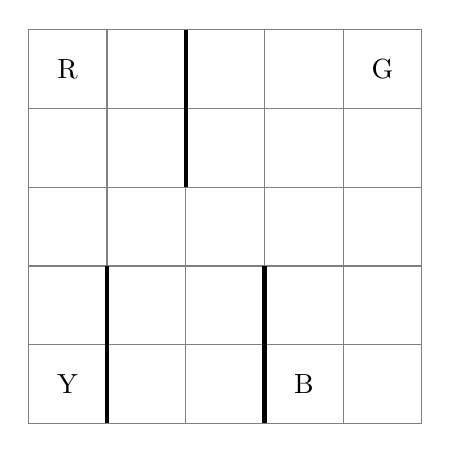
\begin{tikzpicture}
    % Grid
    \draw[step=1,color=gray] (0,0) grid (5,5);
    
    % Walls
    \draw[line width=1.5pt] (2,5) -- (2,3);
    \draw[line width=1.5pt] (1,0) -- (1,2);
    \draw[line width=1.5pt] (3,0) -- (3,2);

    % Pads
    \draw (0.5,4.5) node {R};
    \draw (0.5,0.5) node {Y};
    \draw (3.5,0.5) node {B};
    \draw (4.5,4.5) node {G};
\end{tikzpicture}
\end{document}

      \label{fig:taxi-domain}
    }
    \subfigure{
      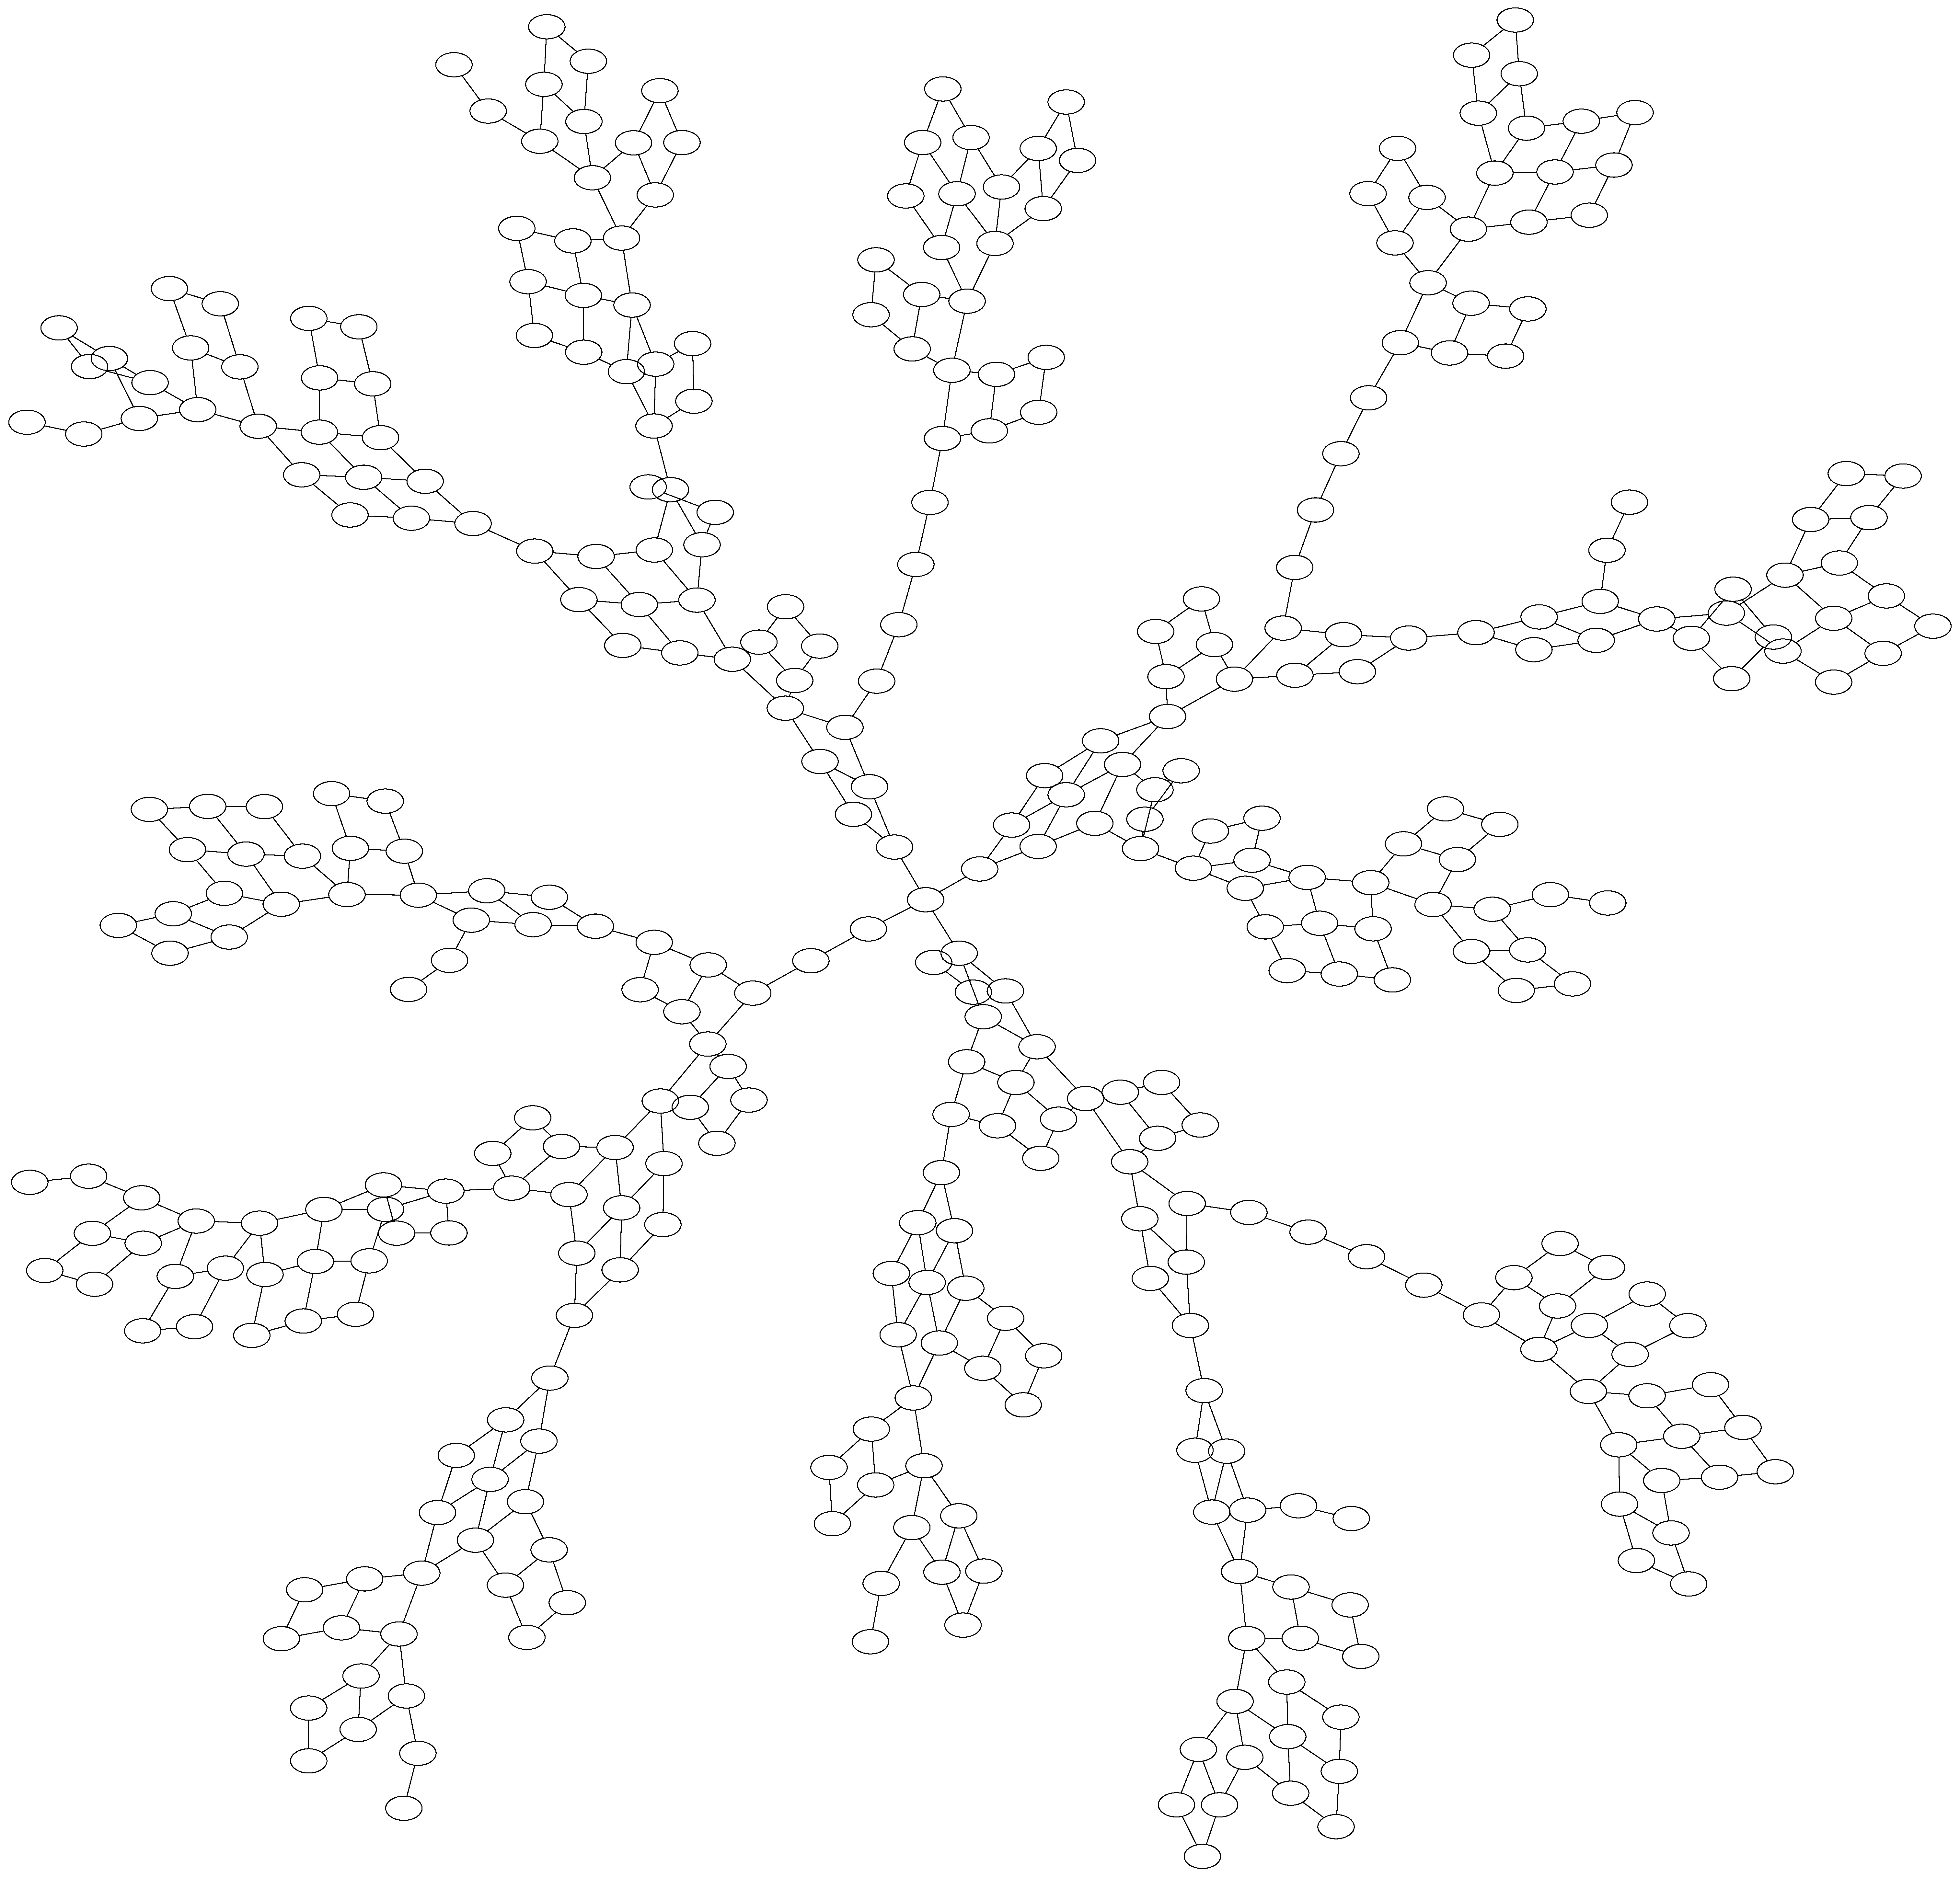
\includegraphics[height=2in]{figures/taxi1}
      \label{fig:taxi-graph}
    }
    \caption{The Taxi Domain, and its State Space Graph}
\end{figure*}

\begin{example}
To make the discussion more tangible, let us look at an example, the
Taxi domain, shown in \figref{fig:taxi-domain}. The agent is a taxi
navigating in this road-map. It must pick up a passenger at one of the
4 pads, A, B, C or D.  Subsequently, it must carry the passenger to a
destination, which is also one of the above four pads. The states of
the taxi would then be a tuple containing the location of the
passenger (in one of the four pads, or within the taxi), the
destination of the passenger, and location of the taxi in the map.
The actions the taxi can perform are moving up, down, left or right in
the map, as well as pick up or drop a passenger at a pad. 
Typical options for such a domain would be an option that can be
started anywhere, and has a policy that takes the taxi to the one of
the pads in the shortest possible manner. Such an option is generic,
and does not depend on where the passenger or destination are. The RL
agent must then learn to choose the right option when picking up the
passenger.
\end{example}


% Prove the interesting result
\section{Small World Options}
\label{sec:theory}

% What are small world options
In Kleinberg's small-world network model, each node $u$ is given one
`long-range' edge to a node $v$, which was chosen with a probability
$P_r(u,v) \propto \|u-v\|^{-r}$, where $\|u-v\|$ denotes the distance
between $u$ and $v$ in the graph. Similarly for each state $s$, we add
a single `path option' to another state $s'$, where $s'$ is chosen with
probability $P_r(s,s') \propto \|s-s'\|^{-r}$. A path option $o_p(s,s')$
is an option with $\initset = \{s\}$, $\stopcond = \{s'\}$, and an
optimal policy to reach $s'$ for $\pi$. Intuitively, it is an option
that takes the agent from $s$ to $s'$. In practice, we may generate path
options only for a subset of $|S|$. Note that while $O(|S|)$ options are
created, only one additional option is available in any state, and thus
the decision-space for the agent is not significantly larger.

% What is the guarantee we give about them?
On an $r$-dimensional lattice, $\klein_r$, the distance from any node
$u$ to a target node $t$ is bounded by $\|u-t\|$, a quantity which is
locally computable. When given long-range edges distributed according to
$P_r$, Kleinberg showed that the greedy distributed algorithm
$\greedyalgo$ that chooses a neighbour $v$ closest to $t$ will reach $t$
with an expected time $O(\log(|V|)^2)$. This follows as a trivial
corollary of the following theorem,

\begin{theorem}
    \label{thm:small-world}
    %
    Let $f : V \to \Re$ be a function embedded on the graph
    $\graph(V,E)$, such that, $\kappa_1 \|u-v\| - c_1 \le \|f(u)
    - f(v)\| \le \kappa_2 \|u - v\| - c_2$, where $0 \le \kappa_1 \le
    \kappa_2$, and $0 \le c_2 \le \frac{c_1}{2}$. Let $M_f$ be the
    global maxima of $f$. Let \egreedyalgo be an $\epsilon$-greedy
    algorithm with respect to $f$, i.e.  an algorithm which chooses with
    probability $1-\epsilon$ to transit to the neighbouring state
    closest to $M_f$, i.e. $N(u) = \argmin_v \|f(v) - f(M_f)\|$.
    
    If $\graph(V,E)$ is $r$-dimensional lattice, and contains a long
    distance edge distributed $P_r$, then \egreedyalgo takes $O( (\log
    |V|)^2 )$ steps to reach $M_f$.
\end{theorem}
\begin{proof}
  The key insight of the proof is that with edges distributed according
  to $P_r$, there will always be edge within the neighbourhood of a node
  to an exponentially smaller neighbourhood of the target. Thus, the
  agent will only require to hop through $\log |V|$ `neighbourhoods'. By
  bounding the time spent in each neighbourhood to $\log |V|$, we arrive
  at the result. We refer the reader to
  \appendixref{sec:small-world-theory} for the complete proof.
\end{proof}

\begin{figure}[th]
    \centering
    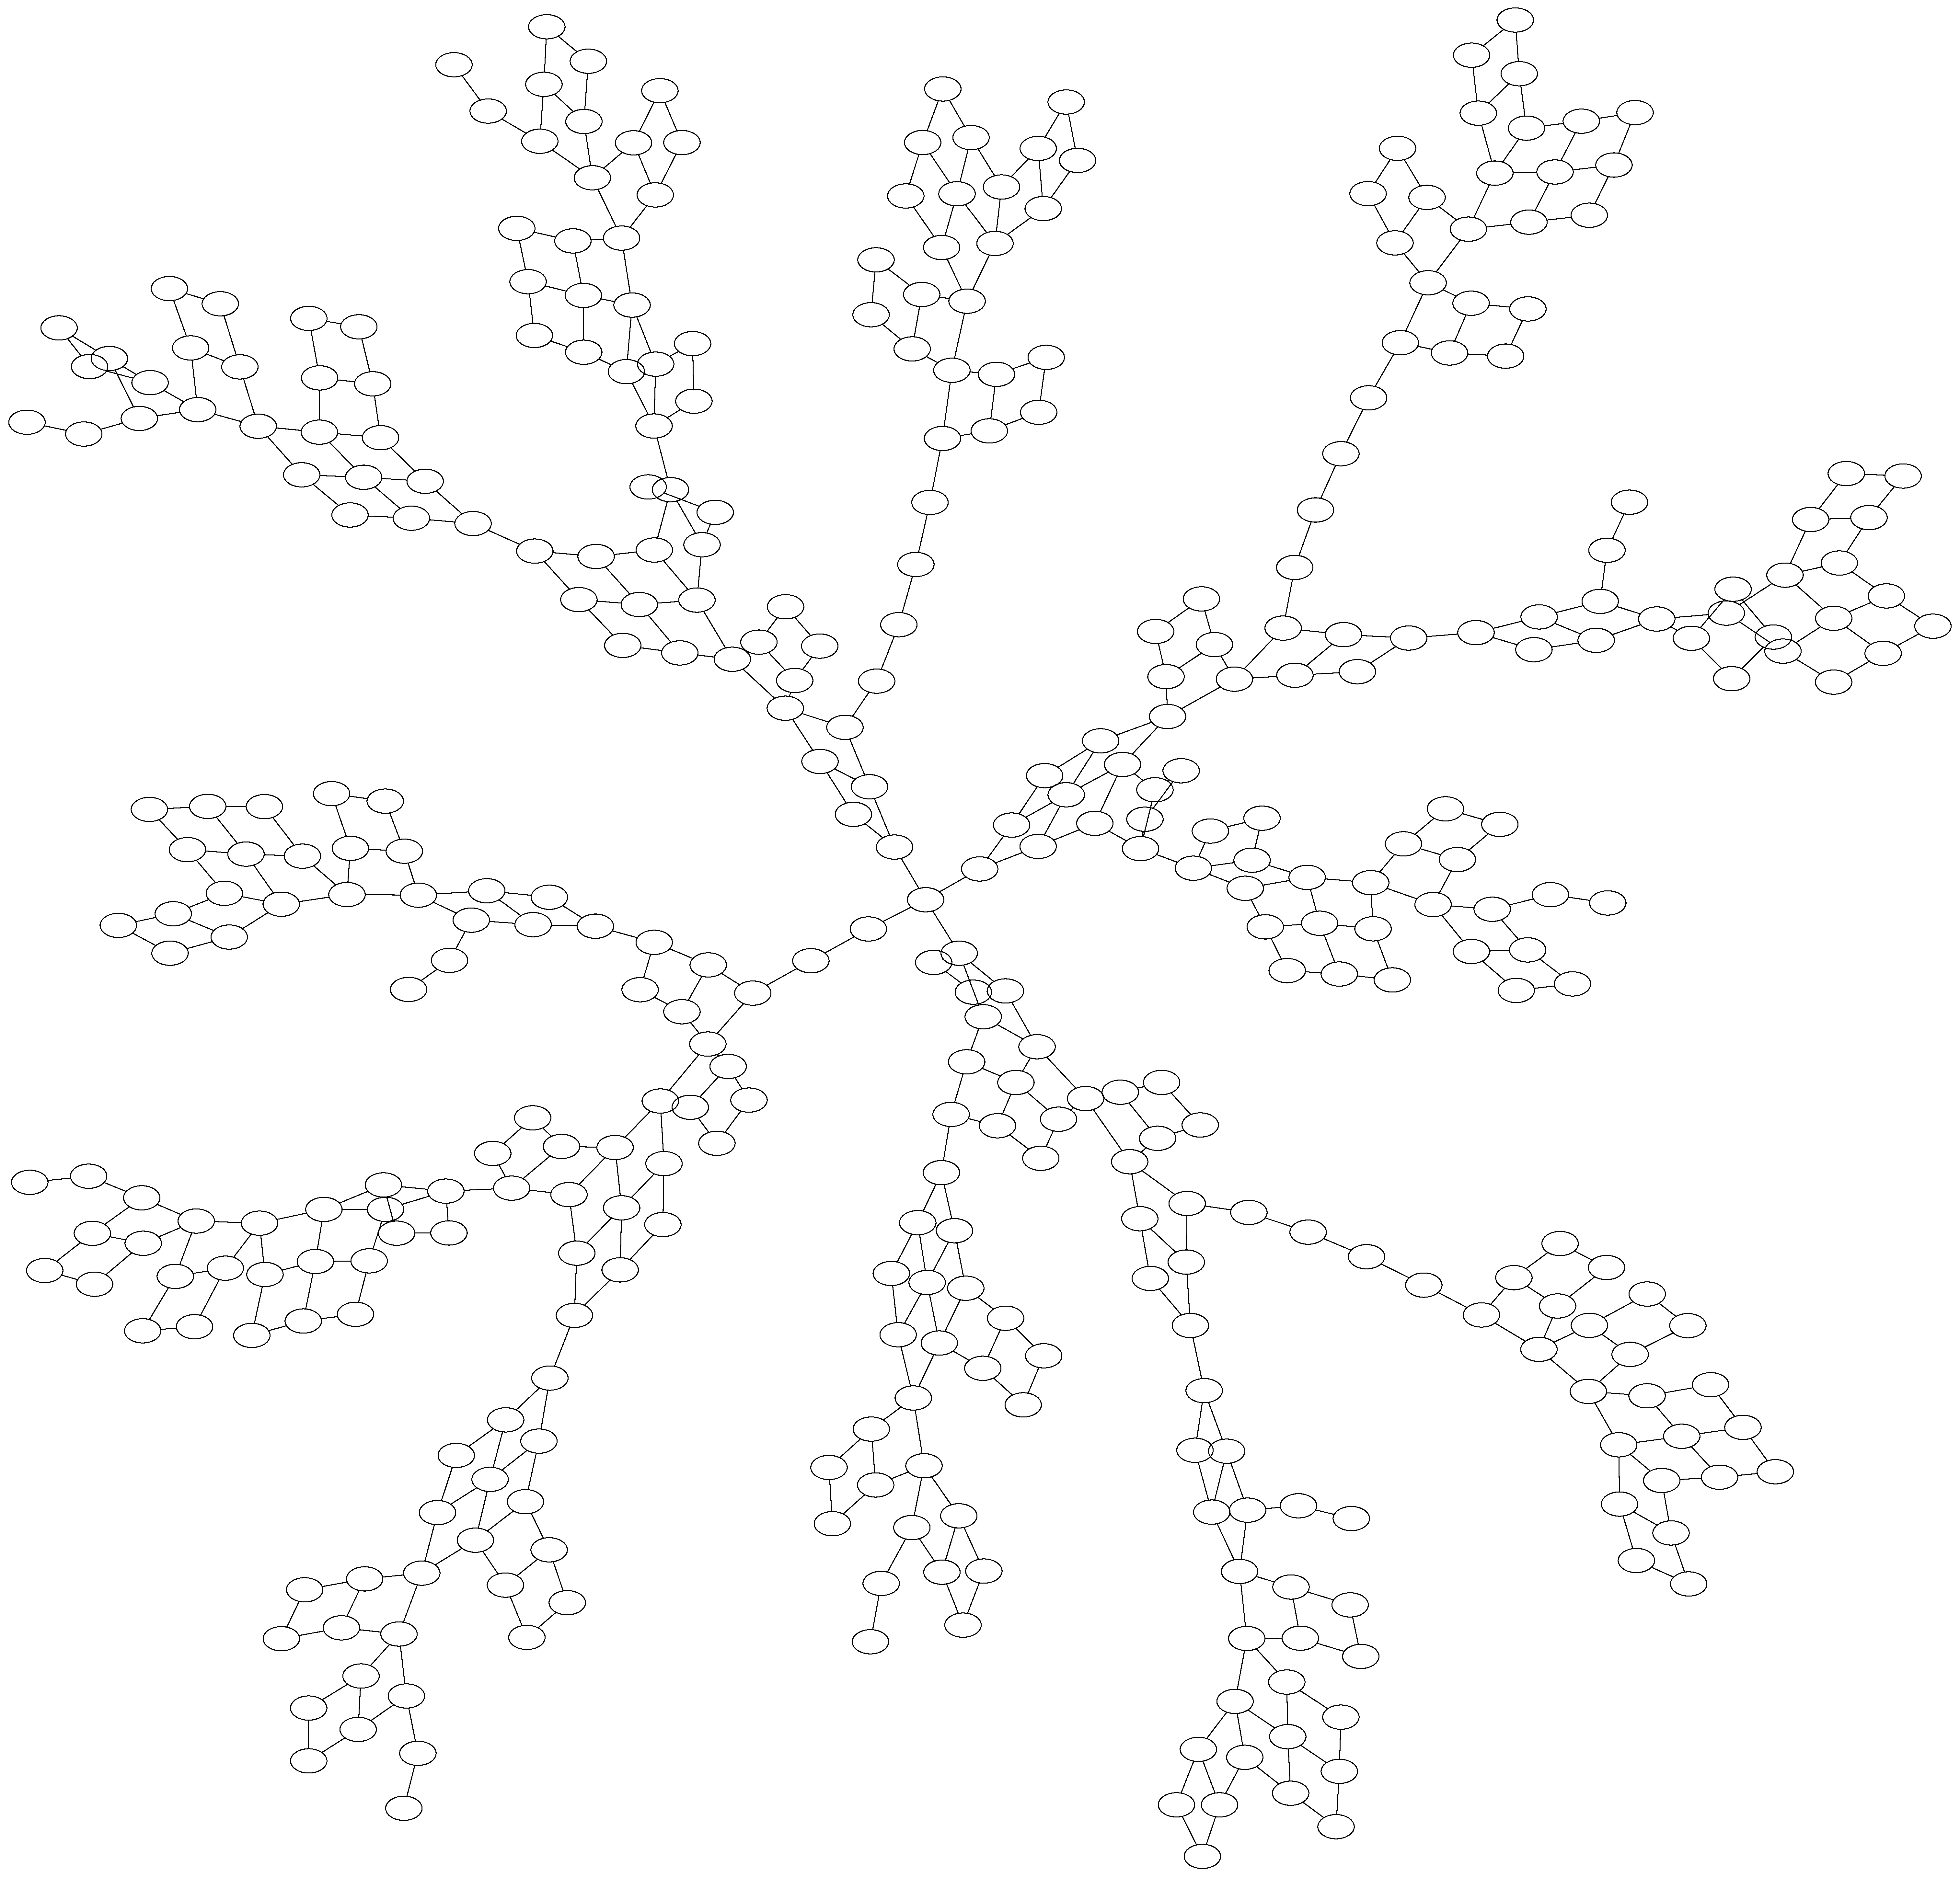
\includegraphics[height=2in]{figures/taxi1}
    \label{fig:taxi-graph}
    \caption{The State Space Graph for Taxi}
\end{figure}

% Graph-based
It is easy to construct a graph $\graph_{\mdp}$ out of the state-space
described by an MDP. The states $\states$ become the nodes of the graph,
and actions $\actions$ become the edges, with the transition
probabilities as weights. The edges can also be attributed with the
rewards described by $\rewards$. Options can be viewed to be paths along
the graph. As an example, the Taxi domain defined earlier translates to
the graph shown in \figref{fig:taxi-graph}.

Consider an MDP $\mdp_{\klein_r}$ with states connected in
a $r$-dimensional lattice, and noisy navigational actions between
states. We claim that using path options distributed according to $P_r$,
an $\epsilon$-greedy agent can reach a state of maximal value using
$O(\log(|S|)^2)$ options. Clearly, the value function $\Vf$ is a local
property of the state. Thus, if we can relate $\Vf$ to the distance from
the target state, we can apply \thmref{thm:small-world}.

\begin{definition}
    A {\em robust path option} $o(u,v)$, where $u,v \in \states$ is an
    option that takes the agent from $u$ to $v$ `robustly', in the
    sense that in each epoch, the agent moves closer to $v$ with a
    probability $1-\epsilon > \frac{1}{2}$. \footnote{This condition
    is equivalent to saying that the option takes the agent from $u$
    to $v$ in finite time, and hence is not particularly strong.}.
    Note that this $\epsilon$ includes any environmental effects as
    well.
\end{definition}

The following lemma shows that $\Vf$ satisfies the properties of a
embedded function required for \thmref{thm:small-world}. 

\begin{lemma}
    \label{lm:distance}
    Let $o(u,v)$ be the preferred option in state $u$, and let $\|u -
    v\|_V = |\log \Vf(v) - \log \Vf(u)|$. Then, 
    \begin{IEEEeqnarray*}{rCCCl}
        k_1 \|u - v\| - c_1 & \le & \|u - v\|_V & \le & k_2 \|u - v\|, 
    \end{IEEEeqnarray*}
    \noindent
    where $k_1 = \log \frac{1}{\gamma} $, $k_2 = \log
    \frac{1}{(1-\epsilon)\gamma}$, and $c_1 = \log
    \frac{1}{1-\gamma}$.
\end{lemma}
\begin{proof}
    For notational convenience, let $\epsilonm = 1 - \epsilon$. From the Bellman optimality condition, we get the value of $o(u,v)$ to be,
    \begin{eqnarray*}
        \Qf(u, o(u,v)) &=& \E_{l}[ \gamma^{l} \Vf(v) + \sum_{i=1}^{l} \gamma^{i-1} r_i ],
    \end{eqnarray*}
    \noindent
    where $l$ is the length of the option, and $r_i$ is the reward
    obtained in the $i$-th step of following the option. 
    
    If o(u,v) is the preferred option in state $u$, then $\Vf(u) =
    \Qf(u, o(u,v))$.  Using the property that $0 \le r_i \le 1$,
    \begin{IEEEeqnarray*}{rCCCl}
        \E_{l}[ \gamma^{l} \Vf(v) ] &\le& \Vf(u) &\le& \E_{l}[ \gamma^{l} \Vf(v) + \sum_{i=1}^{l} \gamma^{i-1}] \\
        \E_{l}[ \gamma^{l} ] \Vf(v) &\le& \Vf(u) &\le& \E_{l}[ \gamma^{l} ] \Vf(v) + \frac{1}{1 - \gamma}. \IEEEyesnumber \label{eq:v-bound}
    \end{IEEEeqnarray*}

    $\E_{l}$ is an expectation over the length of the option. Using
    the property that $o(u,v)$ is robust, we move closer to $v$ with
    probability $\epsilonm$; this is exactly the setting of the
    well-studied gambler's ruin problem, where the gambler begins with
    a budget of $\|u-v\|$, and wins with a probability of $\epsilon$.

    \begin{lemma}
        Consider the gambler's ruin problem where the gambler begins 
        with a budget of $m$, and has a winning probability of $q < \frac{1}{2}$
        (the dealer has a winning probability of $p=1-q$). Let $L$ be
        a random variable for the length of the game. Then, 
        \begin{eqnarray*}
            g_m(x) = \sum_{l=0}^{\infty} P(L = l) x^{l} &=& \frac{1}{\lambda_1^m( x ) + \lambda_2^m( x )},
        \end{eqnarray*}
        \noindent
        where $\lambda_1(x) = \frac{1 + \sqrt{1 - 4pq x^2}}{2px}$, and
        $\lambda_2(x) = \frac{1 - \sqrt{1 - 4pq x^2}}{2px}$.

        Further, when $x \le 1$,
        \begin{IEEEeqnarray*}{rCCCl}
            (px)^m  &\le&  g_m(x) &\le& x^m.
        \end{IEEEeqnarray*}
    \end{lemma}
    \begin{proof}
        For the first part. refer \cite{Feller1968}.

        The second part follows as a corollary, 
        \begin{IEEEeqnarray*}{rCCCl}
            \frac{1}{ (\lambda_1( x ) + \lambda_2( x ) )^{m} }  &\le&  g_m(x) &\le& \sum_{l=m}^{\infty} P(L = l) x^{l} \\
            \frac{1}{(\frac{2}{2px})^m}  &\le&  g_m(x) &\le& \sum_{l=m}^{\infty} P(L = l) x^{m} \\
            (px)^m  &\le&  g_m(x) &\le& x^m.
        \end{IEEEeqnarray*}
    \end{proof}

    In our situation, $p = 1 - \epsilon = \epsilonm > \frac{1}{2}$, $q = \epsilon$, and $m = \|u - v\|$.     
    \begin{IEEEeqnarray*}{rCCCl}
        (\epsilonm \gamma)^{\|u-v\|} &\le& \E_{l}[ \gamma^{l} ] &\le& (\gamma)^{\|u-v\|}.
    \end{IEEEeqnarray*}

    Returning to \eqnref{eq:v-bound},
    \begin{IEEEeqnarray*}{rCCCl}
        \E_{l}[ \gamma^{l} ] \Vf(v) &\le& \Vf(u) &\le& \E_{l}[ \gamma^{l} ] \Vf(v) + \frac{1}{1 - \gamma} \\
        (\epsilonm \gamma)^{\|u-v\|} \Vf(v) &\le& \Vf(u) &\le& \gamma^{\|u-v\|} \Vf(v) + \frac{1}{1 - \gamma} \\
        \|u-v\| \log \frac{1}{\gamma} - \log \frac{1}{1-\gamma} &\le& \|u - v\|_V &\le& \|u-v\| \log (\frac{1}{\epsilonm \gamma}).
    \end{IEEEeqnarray*}

\end{proof}


% Describe the algorithms to; a) generate small world options b)
% extract from learning episodes
\section{Constructing Options from Experience} 
\label{sec:algo}


% Experiment section
\section{Empirical Performance}
\label{sec:experiments}
% Experimental results

% Things to be tested
We evaluated the options defined using our method on the Taxi domain described
in \secref{sec:approach}. We compared the performance of Macro Q learning and
Intra-option Q-learning agents using the following option schemes,
\begin{itemize}
   \item \textbf{Small World} Options were generated randomly connecting two nodes of
       the domain using an inverse square law, as described in
       \secref{sec:approach}, with $r = 2$.
   \item \textbf{Betweenness} Options were generated to take any node to a local maxima
       of the betweenness function.
   \item \textbf{Random} Options were generated by randomly connecting two nodes in the
       domain.
   \item \textbf{Manual} Options were manually defined to take the taxi to one of the
       four pads by the shortest path.
   \item \textbf{None} No options were used.
\end{itemize}

The Intra-option Q-learning algorithm requires that the option policies
themselves be Markov, require that every state that the option can visit be part
of $\initset$. For the experiments using the Intra-option learning algorithm, we
modified the ``Small World'' options slightly such that all nodes along the path
were in the initiation set of the option as well.

% Experimental Parameters
To compare the different approaches, we measuring the ratio of how long the taxi
takes to complete the task to the shortest time possible to complete the task,
and have termed this measure "optimality".  Each experiment was averaged over
$200$ runs, and run for $1500$ episodes. We set $\alpha$ to $0.8$ for all the
experiments. We ran the experiments for two values of $\gamma$, $0.90$ and
$0.99$, with equal performance. We present the results only for $\gamma$ set to
$0.99$.

We plotted the value of optimality versus the number of episodes of the agent,
and have also zoomed into the later episodes to have a closer look at the
converged behaviour.

% Plots
\begin{figure}[ht]
    \centering
    \subfigure[]{
    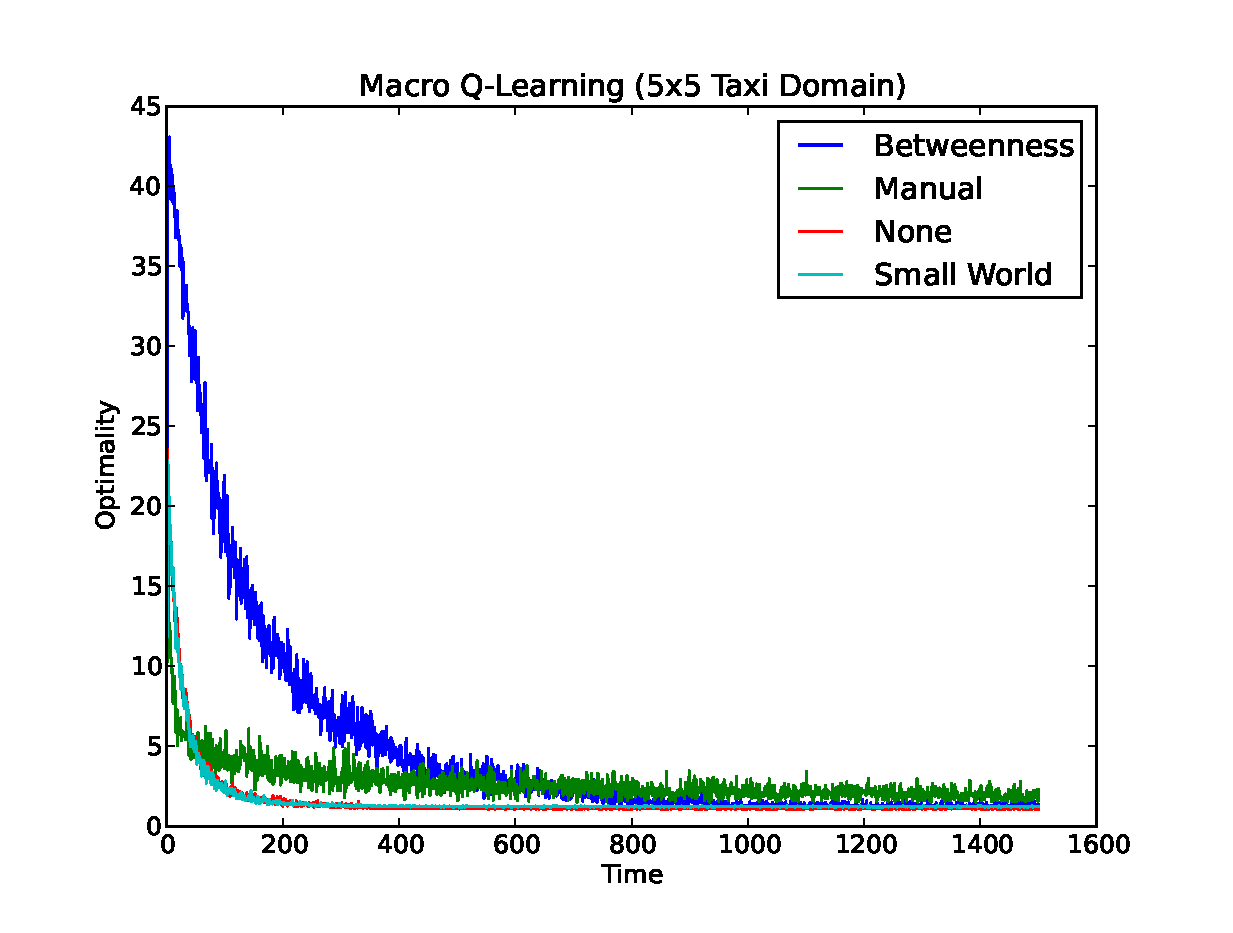
\includegraphics[width=4in]{figures/MacroQ-0_99-taxi1}
    }
    \subfigure[]{
    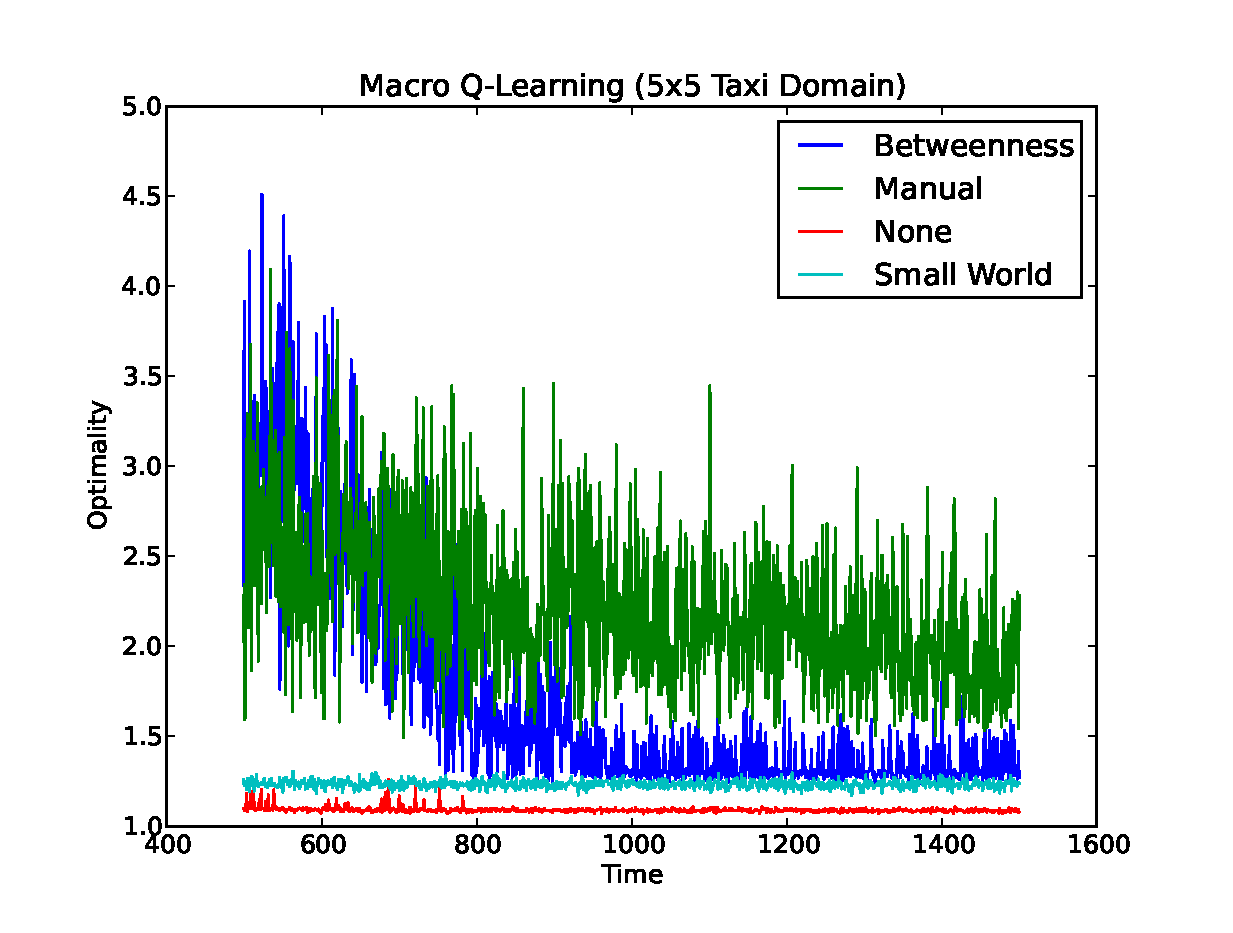
\includegraphics[width=4in]{figures/MacroQ-0_99e-taxi1}
    }
    \caption{Macro Q-learning using 20 options }
    \label{fig:MacroQ-0.99}
\end{figure}

\begin{figure}[ht]
    \centering
    \subfigure[]{
    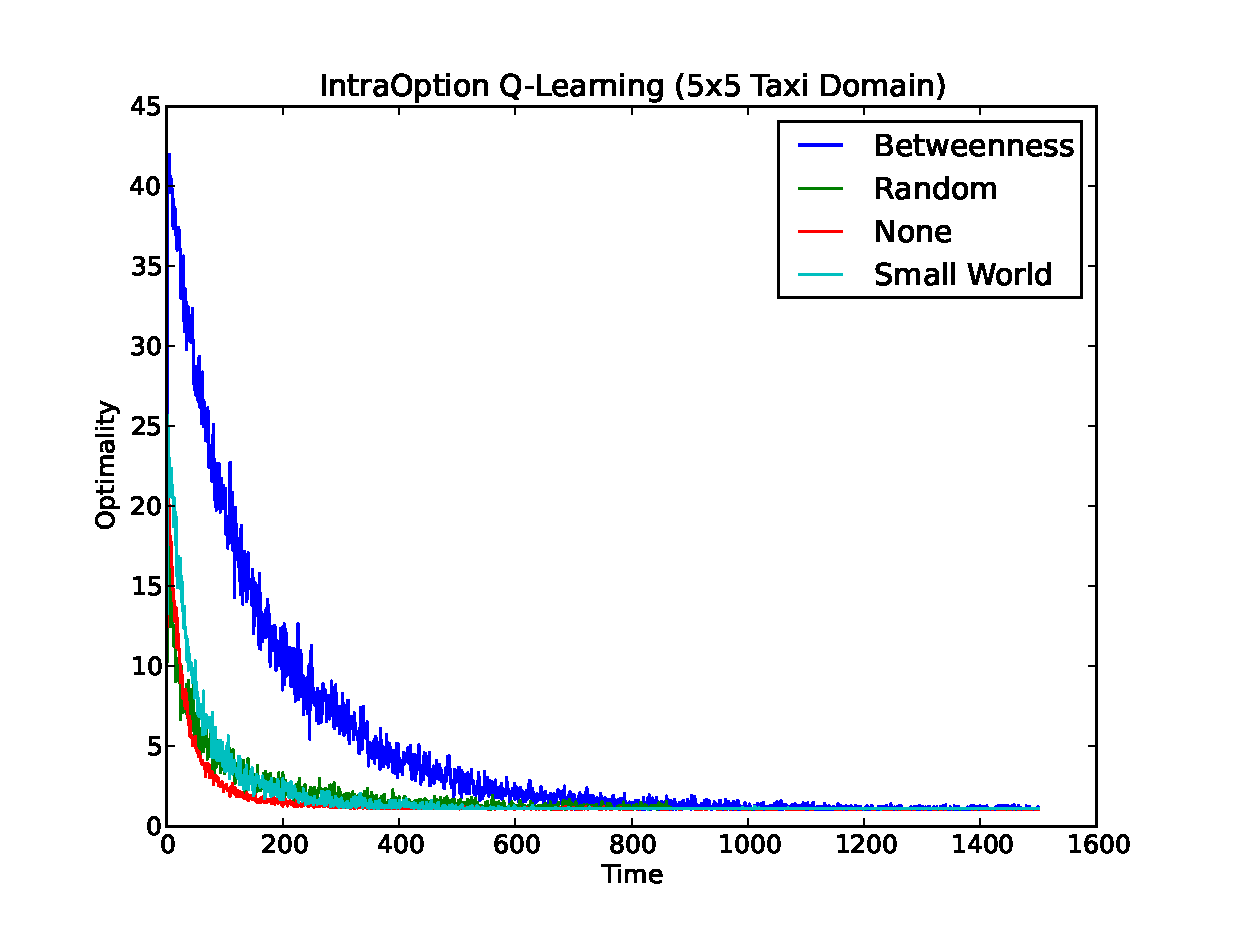
\includegraphics[width=4in]{figures/IntraQm-0_99-taxi1}
    }
    \subfigure[]{
    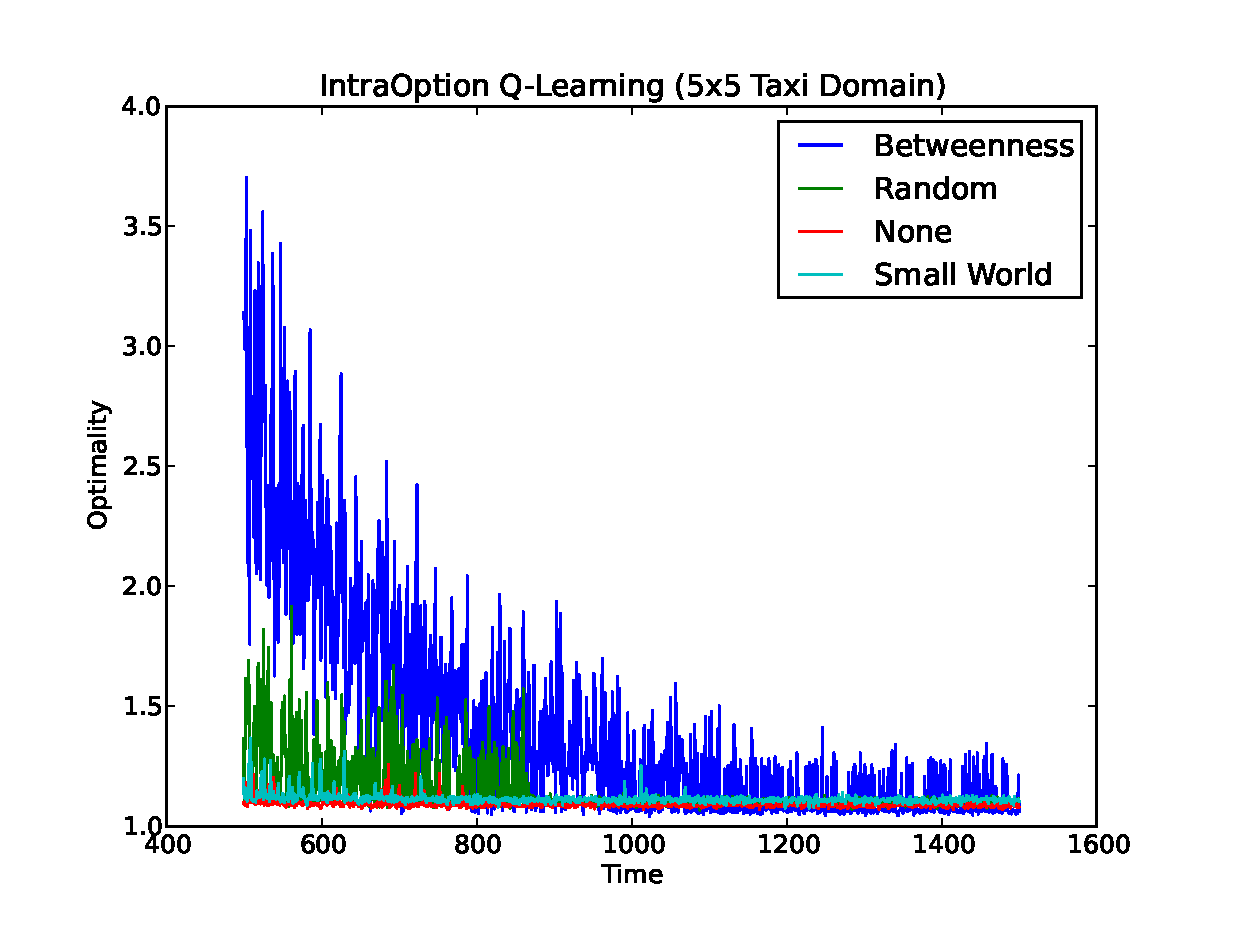
\includegraphics[width=4in]{figures/IntraQm-0_99e-taxi1}
    }
    \caption{Intra-option Q-learning using 20 options }
    \label{fig:IntraQ-0.99}
\end{figure}

\begin{figure}[ht]
    \centering
    \subfigure[]{
    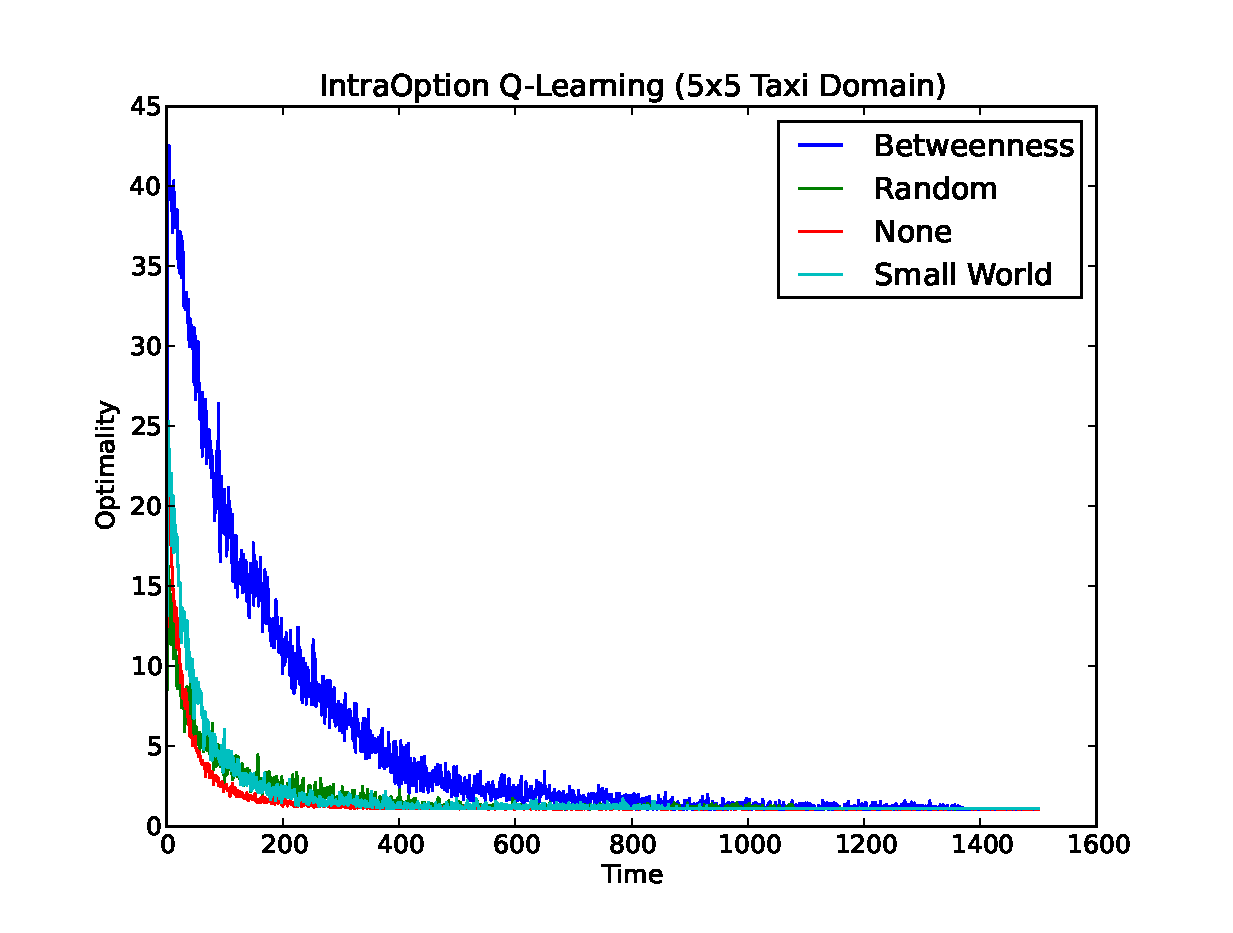
\includegraphics[width=4in]{figures/IntraQm-0_99-50-taxi1}
    }
    \subfigure[]{
    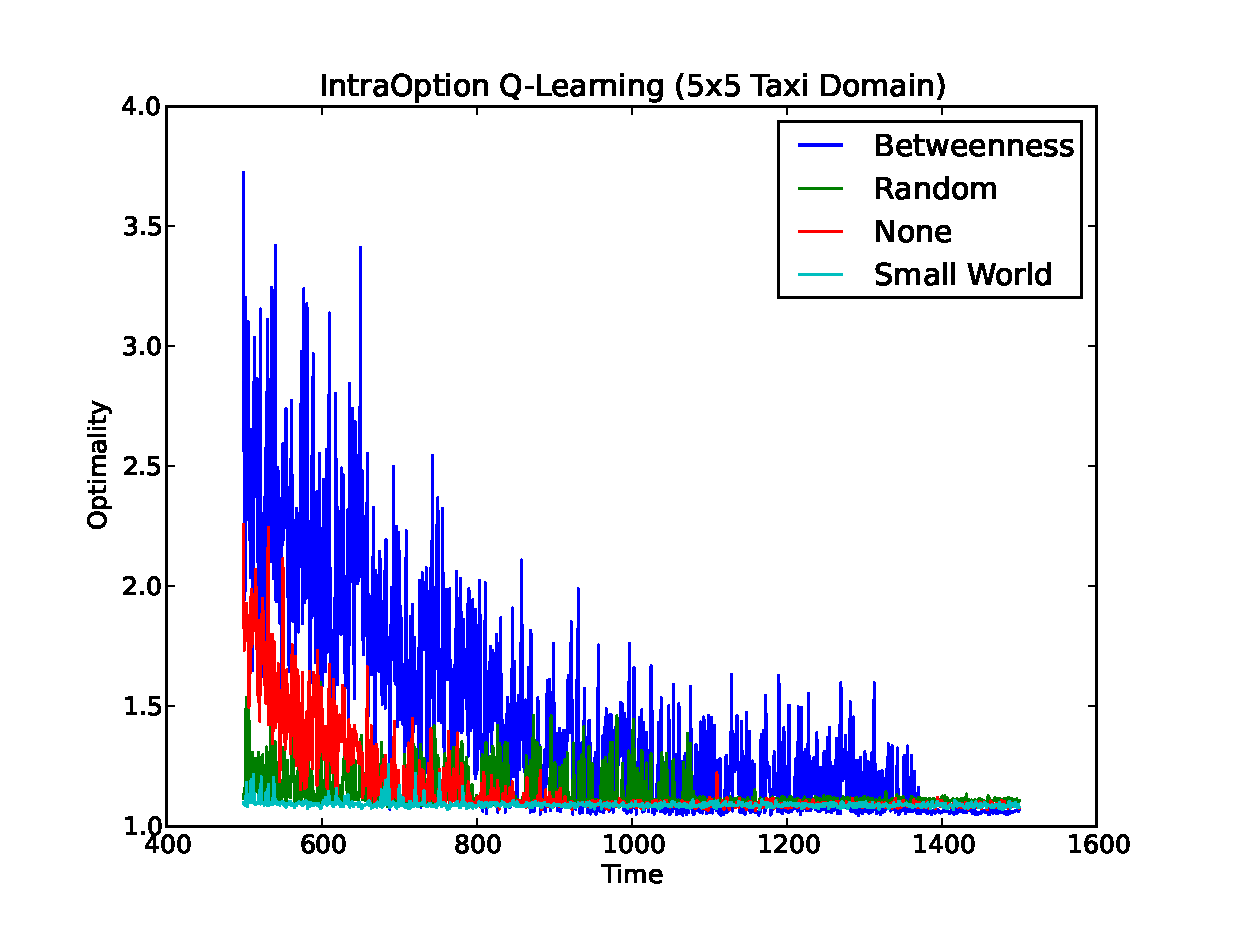
\includegraphics[width=4in]{figures/IntraQm-0_99e-50-taxi1}
    }
    \caption{Intra-option Q-learning, using 50 options }
    \label{fig:IntraQ-0.99-50}
\end{figure}

% Brief on results
We note that the agents using Small World options converge quickly to the
optimal value (i.e. 1), and have small variance. Expectedly, the performance
using Intra-option Q-learning (\autoref{fig:IntraQ-0.99}) is significantly
better than Macro Q-learning (\autoref{fig:MacroQ-0.99}). The performance of
small world options does not significantly differ between using 20 options
(\autoref{fig:IntraQ-0.99}) or 50 options (\autoref{fig:IntraQ-0.99-50}).

We find it surprising that betweenness performs worse than the remaining
schemes. Our options differ from the random options defined in \cite{Simsek} as
we select random paths instead of random nodes to which all other nodes are
connected. As a result, for many nodes there are few if any options. As adding
options also increases the number of actions that an agent can choose from, this
might have lead to the better performance of Random and Small World, which are
both path-based options.

% \begin{table}[ht]
%     \centering
%     \begin{tabular}{ r | r }
%           &  \\ \hline
%           &  \\
%     \end{tabular} 
%     \caption{ }
%     \label{tbl:rtt-summary}
% \end{table}

% \begin{figure}[s]
%     \centering
%     \includegraphics[width=5in]{filename}
%     \caption{ }
%     \label{fig:high-variance-rtt}
% \end{figure}


% Discuss conclusions
\section{Conclusions and Future Work}
\label{sec:conclusions}

% Contributions
% - new scheme for generating options
We have devised a new scheme to generate options based on small world
network model. The options generated satisfy an intuitive criteria, that
the subtasks learnt should be easily composed to solve any other task.
The options also greatly improve the connectivity properties of the
domain.

% - absolutely model-free
Experiments run on standard domains show significantly faster learning
rates using small world options. At the same time, we have shown that
learning small world options can be significantly cheaper than learning
`bottleneck' options. Another advantage of the scheme is that is does
not ever require the model of the MDP. We find it remarkable that we can
learn near optimal behaviour just from the policies of on some tasks


% - theoretical interest
The scheme does not perform any global analysis, and does not require
the model. We have shown that sample-wise, it can be far cheaper than
other bottleneck based methods. Does not lead to state space blow up.
Also is interesting from a theoretical perspective, logarithmic number
of decisions.

% Further work
% - dynamically add/remove options
% - figuring out r
We have as yet not been able to characterise what the exponent $r$
should be in a general domain. Given the ease with which options can be
discovered, it would be interesting to create a dynamic scheme.



\bibliographystyle{abbrv}
\bibliography{ref}{}

%\balancecolumns

\appendix
\section{Small Worlds}
\label{sec:small-worlds}

% Introduction and motivation for the proof
In this section, we will prove that the number of decisions taken by
an $\epsilon$-greedy agent, $\egreedyalgo$, to reach a maximal value
state in a $k$-dimensional lattice $\graph_k(V,E)$ is $O( (\log
V)^2)$. This is a simple extension to the Kleinberg's result. Our
approach is similar to that of Kleinberg's \cite{Kleinberg}, though we
adopt the somewhat cleaner notation of \cite{Martel2004}.

% Abstract result
Consider a $k$-dimensional lattice $\graph_k(V,E)$ with random links distributed
according to an inverse power law distribution $p(u,v) \propto \|u-v\|^{-k}$,
where $\|u - v\|$ is the distance between $u$ and $v$ in $\graph$. 

\begin{definition}
Let us define $\ball_l(u)$ to be the set of nodes contained within a
``ball'' of radius $l$ centered at $u$, i.e.  $\ball_l(u) = \{ v \mid
\|u - v\| < l \}$, and $\sball_l(u)$ to be the set of nodes on its
surface, i.e. $\sball_l(u) = \{ v \mid \|u - v\| = l \}$.
\end{definition}

We begin by finding the normalisation constant for the probability
distribution $p(u,v)$.

\begin{lemma}
    The inverse normalised coefficient for $p(u,v)$ is $c_u = \theta(
    \log n )$, and $p(u,v) = \|u - v\|^{-k} \theta( (\log n)^{-1} )$.
\end{lemma}
\begin{proof}
    \begin{eqnarray*}
        c_u &=& \sum_{v \ne u} \|u - v\|^{-k} \\
            &=& \sum_{j=1}^{k(n-1)} \sball_j(u) j^{-k}.
    \end{eqnarray*}
    It can easily be shown that the $\sball_l(u) = \theta( l^{k-1} )$.
    Thus, the $c_u$ reduces to a harmonic sum, and hence, $c_u =
    \theta( \log n )$.  The second part of the lemma follows as
    $p(u,v) = \frac{ \|u - v\|^{-k} }{c_u}$. 
    \\ \qed
\end{proof}

Now, consider a function $f$ embedded on $\graph(V,E)$, i.e. $f : V
\to \Re$, with the property that $\kappa_1 \|u-v\| - c_1 \le \|f(u) -
f(v)\| \le \kappa_2 \|u - v\| - c_2$, where $0 \le \kappa_1 \le
\kappa_2$, and $0 \le c_2 \le \frac{c_1}{2}$. Equivalently,
$\frac{\|f(u)-f(v)\| + c_2}{\kappa_2} \le \|u - v\| \le
\frac{\|f(u)-f(v)\| + c_1}{\kappa_1}$. We analogously define
$\ballf_l(u) = \{ v \mid \|f(u) - f(v)\| < l \}$. Let $M_f$ be the
global maxima of $f$. For notational convenience, we take $\ballf_l$
to be $\ballf_l(M_f)$.

% Describe problem / algo
\begin{definition}
    Let $\egreedyalgo$ be an $\epsilon$-greedy algorithm. If $N(u)$ is
    the next node chosen by $\egreedyalgo$, then $\egreedyalgo$
    chooses with probability $1-\epsilon$, the edge $(u,v)$ such that
    the distance of $v$ from the global maxima is minimum, i.e. $N(u)
    = \argmin_v \|v - f(M_f)\|$.
\end{definition}

We are now ready to prove the following general result.

\begin{theorem}
    \label{thm:decisions}
    \egreedyalgo takes $O( (\log n)^2 )$ decisions.
\end{theorem}
\begin{proof}
    Let a node $u$ be in phase $j$ when $u \in \ballf_{2^{j+1}}
    \setminus \ballf_{2^{j}}$. The probability that phase $j$
    will end this step is equal to the probability that $N(u) \in
    \ballf_{2^{j}}$. 
    
    The size of $\ballf_{2^{j}}$ is at least $|\ball_{\kappa_2^{-1}(
    2^{j}+c_2)}| = \theta( \kappa_2^{-k} (2^{j}+c_2)^{k} )$. The
    distance between $u$ and a node in $\ballf_{2^{j}}$ is at most
    $\frac{2^{j+1} + c_1}{ \kappa_1 } + \frac{2^{j} + c_2}{\kappa_2} <
    2(\frac{2^{j+1} + c_2}{\kappa_2})$. The probability of a link
    between these two nodes is at least $\kappa_1^{-k} (2^{j+2} + 2
    c_1)^{-k} \theta(\log n)^{-1} $. Thus, 

    \begin{eqnarray*}
        P(u, \ballf_{2^{j}} ) &\ge& (1-\epsilon) (\frac{2^{j}+c_2}{\kappa_2})^{k} \times (\frac{2^{j+2} + 2 c_1}{\kappa_1})^{-k} \theta( \log n )^{-1}  \\
        &\ge& \frac{(1-\epsilon)}{\theta( \log n )} \times (\frac{\kappa_1}{4\kappa_2} )^{k} \times ( \frac{ 1 + \frac{c_2}{2^{j}} }{ 1 + \frac{c_1}{2 \times 2^{j}} })^{k}\\
        &\ge& \frac{(1-\epsilon)}{\theta( \log n )} \times (\frac{\kappa_1}{4\kappa_2} )^{k} \times ( \frac{ 1 + c_2 }{ 1 + \frac{c_1}{2} })^{k} .\\
    \end{eqnarray*}

    Let number of decisions required to leave phase $j$ be $X_j$. Then, 
    \begin{eqnarray*}
        \E[X_j] &\le& \sum_{i=0}^{\infty} (1 - P(u, \ballf_{2^{j}} ))^i \\
                &\le& \frac{1}{P(u, \ballf_{2^{j}} )} \\
                &\le& \theta( \log n ) \frac{1}{(1-\epsilon)} (\frac{4 \kappa_2}{\kappa_1})^{k} ( \frac{ 1 + \frac{c_1}{2} }{ 1 + c_2 })^{k}\\
                &\le& \theta( \log n ).
    \end{eqnarray*}
    Thus, $\E[X_j]$ is $O(\log n)$. By construction, there are at most $\log n$
    phases, and thus at most $O((\log n)^2)$ decisions.
    \\ \qed
\end{proof}


%\balancecolumns 

\end{document}

